\documentclass[../Book.tex]{subfiles}
 
\begin{document}
	\section{Gambaran Umum Sistem}
	Tujuan dari sistem yang dibangun adalah untuk mencari tindak plagiat yang ada pada dua buah dokumen dengan metode \textit{Merging Context Seeds}. Alur secara umum yang ada pada sistem ditunjukan pada Gambar \ref{fig:gambarumumsistem} dimana titik awal sistem bekerja berdasarkan \textit{pairs} dan hasil akhir adalah bagian pada teks yang melakukan plagiat.
	
	\begin{center}
		\begin{figure}[H]
			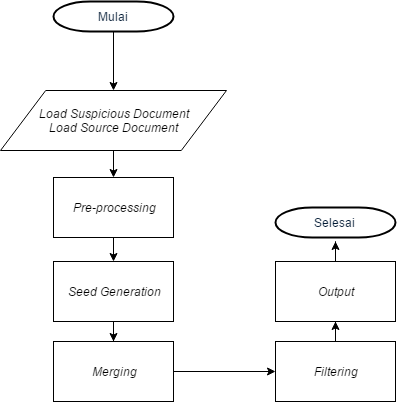
\includegraphics[width=.7\linewidth]{../images/flowchart}
			\caption{Gambaran Umum Sistem}
			\label{fig:gambarumumsistem}
		\end{figure}
	\end{center} 
	
	\noindent \textbf{\textit{Load document}} \\
	Dari satu buah \textit{pair}, akan dimuat 2 buah dokumen yaitu \textit{suspicious-document} (Dokumen X) dan \textit{source-document} (Dokumen Y) yang merupakan \textit{plain text} yang berisikan sebuah artikel. \\
	
	\noindent Untuk \textit{pre-processing, seed generation, merging, filtering, }dan \textit{output} dijelaskan pada Sub-Bab 3.3
	
\end{document}